%%%%%%%%%%%%%%%%%%%%%%%%%%%
%%%%% DOCUMENT FORMAT %%%%%
%%%%%%%%%%%%%%%%%%%%%%%%%%%

%%%%%%%%%%%%%%%%%%%%%%%%%%%%%%%%%%%%%%%%%%%%%%
%%%%% Converting this document to PDF %%%%%%%%
%%%%%%%%%%%%%%%%%%%%%%%%%%%%%%%%%%%%%%%%%%%%%%

%% See  http://cxc.harvard.edu/proposer/generatePDF.html

\documentclass[letterpaper,11pt,twocolumn]{article}
%\documentclass[letterpaper,11pt]{article}

%%%%%%%%%%%%%%%%%%%%%%%%%%%%%
%%%%% Included packages %%%%%
%%%%%%%%%%%%%%%%%%%%%%%%%%%%%

\usepackage{graphics,graphicx}
\usepackage{amssymb,comment}
\usepackage{wrapfig,natbib,aastex_hack}
\usepackage{xcolor,setspace,tikz}
\usepackage{siunitx}

\def\la{\mathrel{\hbox{\rlap{\hbox{\lower4pt\hbox{$\sim$}}}\hbox{$<$}}}}
\def\ga{\mathrel{\hbox{\rlap{\hbox{\lower4pt\hbox{$\sim$}}}\hbox{$>$}}}}
\def\arcdeg{\hbox{$^\circ$}}
\def\arcmin{\hbox{$^\prime$}}
\def\arcsec{\hbox{$^{\prime\prime}$}}

%%%%%%%%%%%%%%%%%%%%%%%%%%%
%%%%% Page dimensions %%%%%
%%%%%%%%%%%%%%%%%%%%%%%%%%%

\setlength{\textwidth}{6.5in} 
\setlength{\textheight}{9in}
\setlength{\topmargin}{-0.0625in} 
\setlength{\oddsidemargin}{0in}
\setlength{\evensidemargin}{0in} 
\setlength{\headheight}{0in}
\setlength{\headsep}{0in} 
\setlength{\hoffset}{0in}
\setlength{\voffset}{0in}


%%%%%%%%%%%%%%%%%%%%%%%%%%%%%%%%%%%%%
%%%%% Some Useful Abbreviations %%%%% 
%%%%%%%%%%%%%%%%%%%%%%%%%%%%%%%%%%%%%
\newcommand{\chandra}{{\it Chandra}}
\newcommand{\rxte}{{\it RXTE}}
\newcommand{\asca}{{\it ASCA}}
\newcommand{\rosat}{{\it ROSAT}}
\newcommand{\einstein}{{\it EINSTEIN}}
\newcommand{\ginga}{{\it GINGA}}
\newcommand{\bbxrt}{{\it BBXRT}}
\newcommand{\suzaku}{{\it Suzaku}}
\newcommand{\xmm}{{\it XMM-Newton}}
\newcommand{\sax}{{\it BeppoSAX}}
\newcommand{\ec}{$\eta$~Car}
\newcommand{\glast}{{\it GLAST}}
\newcommand{\swift}{{\it Swift}}
\newcommand{\integral}{\textit{INTEGRAL}}
\newcommand{\nustar}{\textit{NuSTAR}}
\newcommand{\hst}{{\it HST}}
\newcommand{\hitomi}{{\it Hitomi}}
\newcommand{\xrism}{{\it XRISM}}
\newcommand{\ms}{$M_{\odot}$}
\newcommand{\rs}{$R_{\odot}$}
\newcommand{\ls}{$L_{\odot}$}
\newcommand{\kms}{km~s$^{-1}$}
\newcommand{\fluxcgs}{ergs~s$^{-1}$~cm$^{-2}$}
\newcommand{\lumcgs}{ergs~s$^{-1}$}
\newcommand{\ug}{$\mu$G}
\newcommand{\nusky}{{\tt nuskybgd}}
\newcommand{\heasoft}{{\tt HEASoft}}
\newcommand{\xspec}{{\tt XSpec}}
\def\la{\mathrel{\hbox{\rlap{\hbox{\lower4pt\hbox{$\sim$}}}\hbox{$<$}}}}
\def\ga{\mathrel{\hbox{\rlap{\hbox{\lower4pt\hbox{$\sim$}}}\hbox{$>$}}}}
\def\lesssim{\mathrel{\spose{\lower 3pt\hbox{$\mathchar"218$}}
     \raise 2.0pt\hbox{$\mathchar"13C$}}}
\def\gtrsim{\mathrel{\spose{\lower 3pt\hbox{$\mathchar"218$}}
     \raise 2.0pt\hbox{$\mathchar"13E$}}}
\def\arcdeg{\hbox{$^\circ$}}
\def\arcmin{\hbox{$^\prime$}}
\def\arcsec{\hbox{$^{\prime\prime}$}}
\newcommand*\circled[1]{\tikz[baseline=(char.base)]{
            \node[shape=circle,draw,inner sep=2pt] (char) {#1};}}
\newcommand{\todo}[1]{\Large{$\bullet$}\normalsize{(\textcolor{red}{#1})}\Large{$\bullet$}\normalsize{}}
\newcommand{\badtext}[1]{$\rightarrow$(\textcolor{red}{rewrite}) {#1} (\textcolor{red}{rewrite})$\leftarrow$}


%%%%%%%%%%%%%%%%%%%%%%%%%%%%%
%%%%%%%%%% Title %%%%%%%%%%%%
%%%%%%%%%%%%%%%%%%%%%%%%%%%%%

\title{\LARGE \bf
Composition and X-Ray Spectrum of NGC 3516
}

%\author{ \parbox{3 in}{\centering Narshion Ngao*
%         \thanks{*Use the $\backslash$thanks command to put information here}\\
%         Msc. Computer Systems - 2018\\
%         Jomo Kenyatta University of Agriculture \& Technology \\
%       
%}}

\author{Wik PHYS 5590 Spring 2020, Pierce Jorgensen
}

\date{April 30 2020}

%%%%%%%%%%%%%%%%%%%%%%%%%%%%%%%%%%
%%%%% Section heading format %%%%%
%%%%%%%%%%%%%%%%%%%%%%%%%%%%%%%%%%

\makeatletter
\renewcommand{\section}{\@startsection%
{section}{1}{0mm}{-\baselineskip}%
{0.5\baselineskip}{\normalfont\Large\bfseries}}%
\makeatother

%%%%%%%%%%%%%%%%%%%%%%%%%%%%%
%%%%% Start of document %%%%% 
%%%%%%%%%%%%%%%%%%%%%%%%%%%%%

\begin{document}
\pagestyle{plain}
\pagenumbering{arabic}


\maketitle
\thispagestyle{empty}
\pagestyle{empty}


%%%%%%%%%%%%%%%%%%%%%%%%%%%%%
%%%%%%%% Abstract %%%%%%%%%%% 
%%%%%%%%%%%%%%%%%%%%%%%%%%%%%


\section{Abstract}

This report is an exploration into data analysis using the HEASARC Archive and NuSTAR data sets. There is some background information on Active Galactic Nuclei and a Literature Review of some prominent papers on the object NGC 3516. It is an extremely variable and active galaxy that emits mostly in the UV and X-Ray spectrum, while also having some abnormal structural characteristics and suspected outflow-driven shock wave fronts due to synchrotron emission. The X-ray fluctuations are given an attempt at an explanation and some simplified steps of performing data analysis using Heasoft-6.27.2. While many errors were encountered during the use of nupipeline and CALDB, the final products of data analysis from the TAR archive are attached to this report.



%%%%%%%%%%%%%%%%%%%%%%%%%%%%%
%%%%%%% Citations %%%%%%%%%%%
%%%%%%%%%%%%%%%%%%%%%%%%%%%%%

% {\it \citet{MWP+17}}  
% {\it \citet{EN+18}}  137
% {\it \citet{H+19}} 
% {\it \citet{TKM+19}}
% {\it \citet{F+8}} 4749


%%%%%%%%%%%%%%%%%%%%%%%%%%%%%
%%%%%%%% Introduction %%%%%%% 
%%%%%%%%%%%%%%%%%%%%%%%%%%%%%

\section{Introduction}

\subsection{Data Analysis}

NGC 3516 is an incredibly bright lenticular Seyfert I type galaxy in the Ursa Major constellation. It is approximately 38 mega-parsecs away and 20,000 kilo-parsecs across. It is located at right ascension $\alpha$=11h 6m 30s, and declination $\delta$=72\si{\degree} 34' by the equatorial coordinate system. From observations in the radio wave and optical spectrums, long one-sided structures appear from the galactic nucleus extending up to 4 kpc away {\it \citet{MWP+17}}. It is speculated that these structures are synchrotron emissions from the quasar outflow of an active galactic nucleus. They are shaped like this and moving away from the galactic center and perpendicular to the direction of emission due to "outflow-driven shock waves" (4). There also appears to be a rather narrow bean of photoionized radiation from surrounding interstellar gas, which is similar to a blazar.

\begin{figure*}[t]
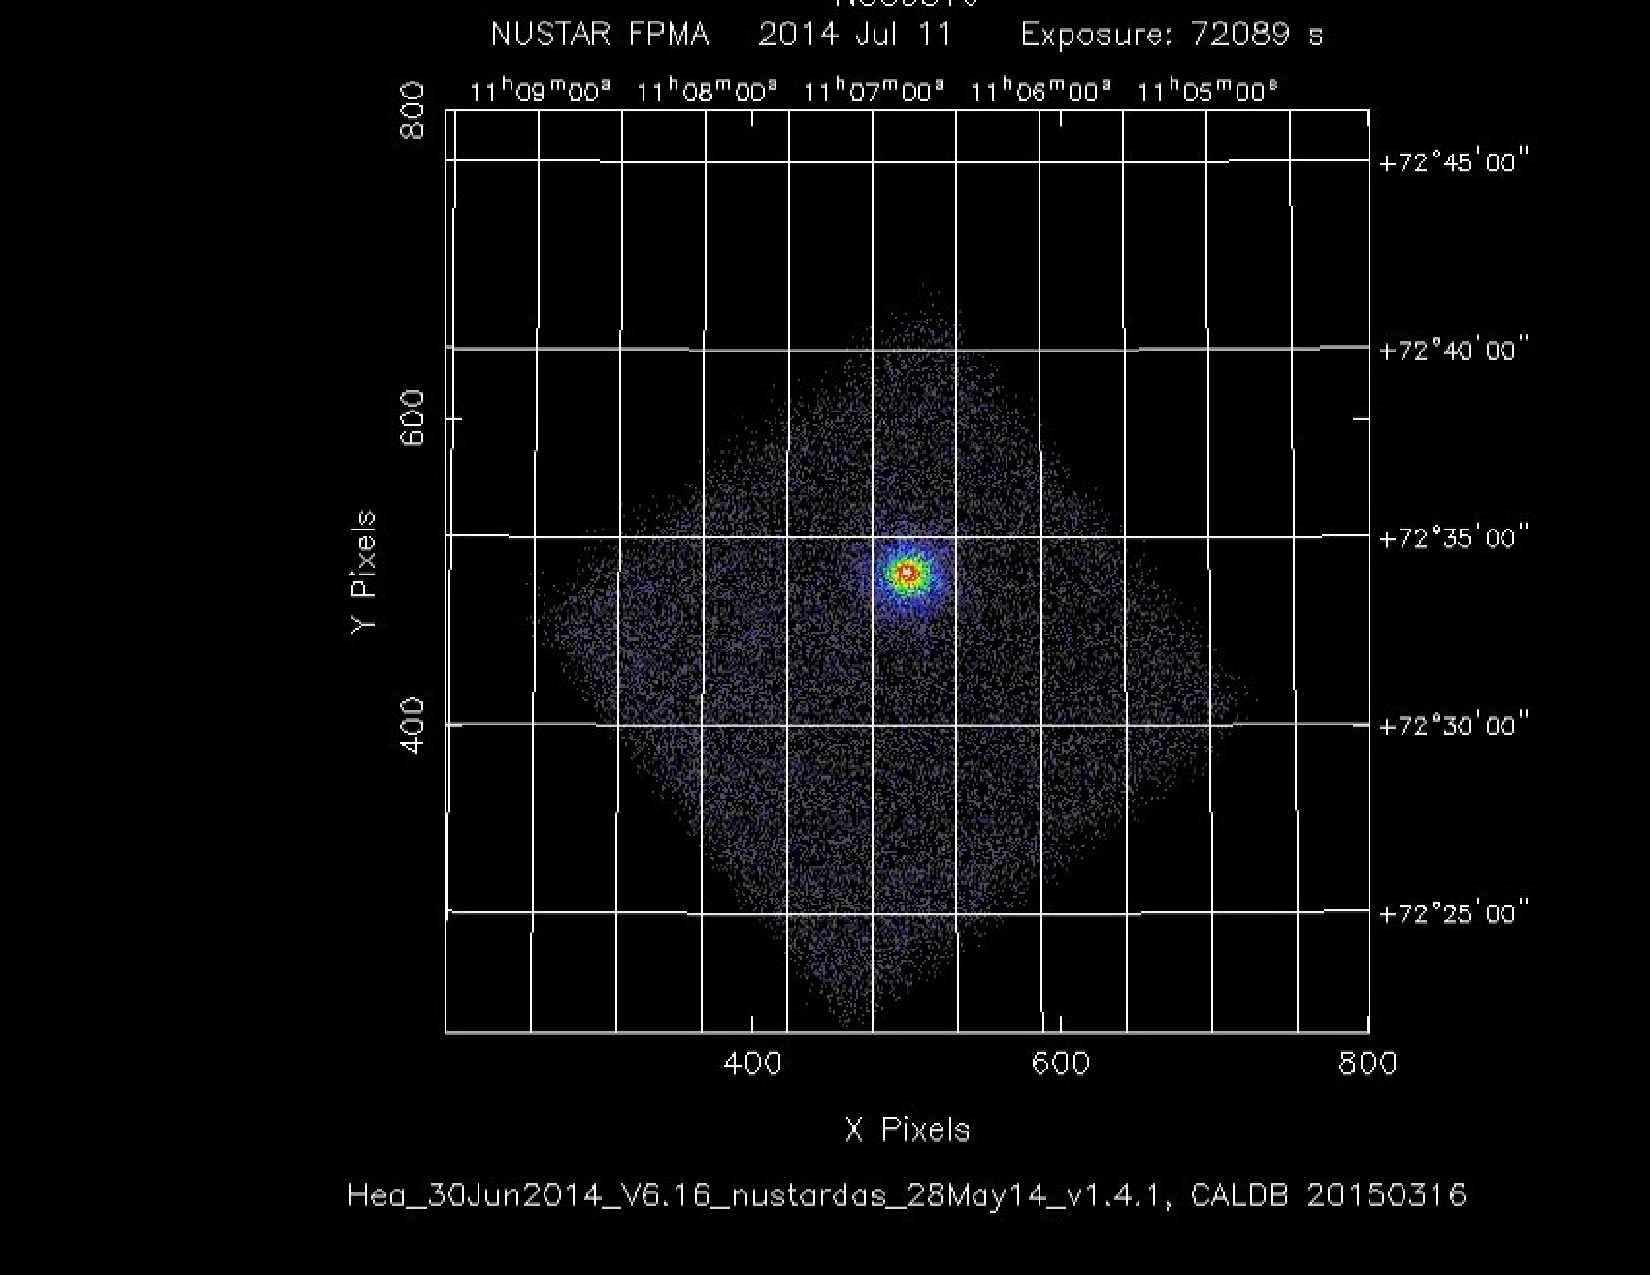
\includegraphics[width=0.7\textwidth]{Images/Image_A.pdf} 
\caption{
2014 X-Ray Band exposure of NGC3516 {\it \citet{H+19}}
\label{fig:Image_B.gif}
}
\end{figure*}

\begin{figure*}[t]
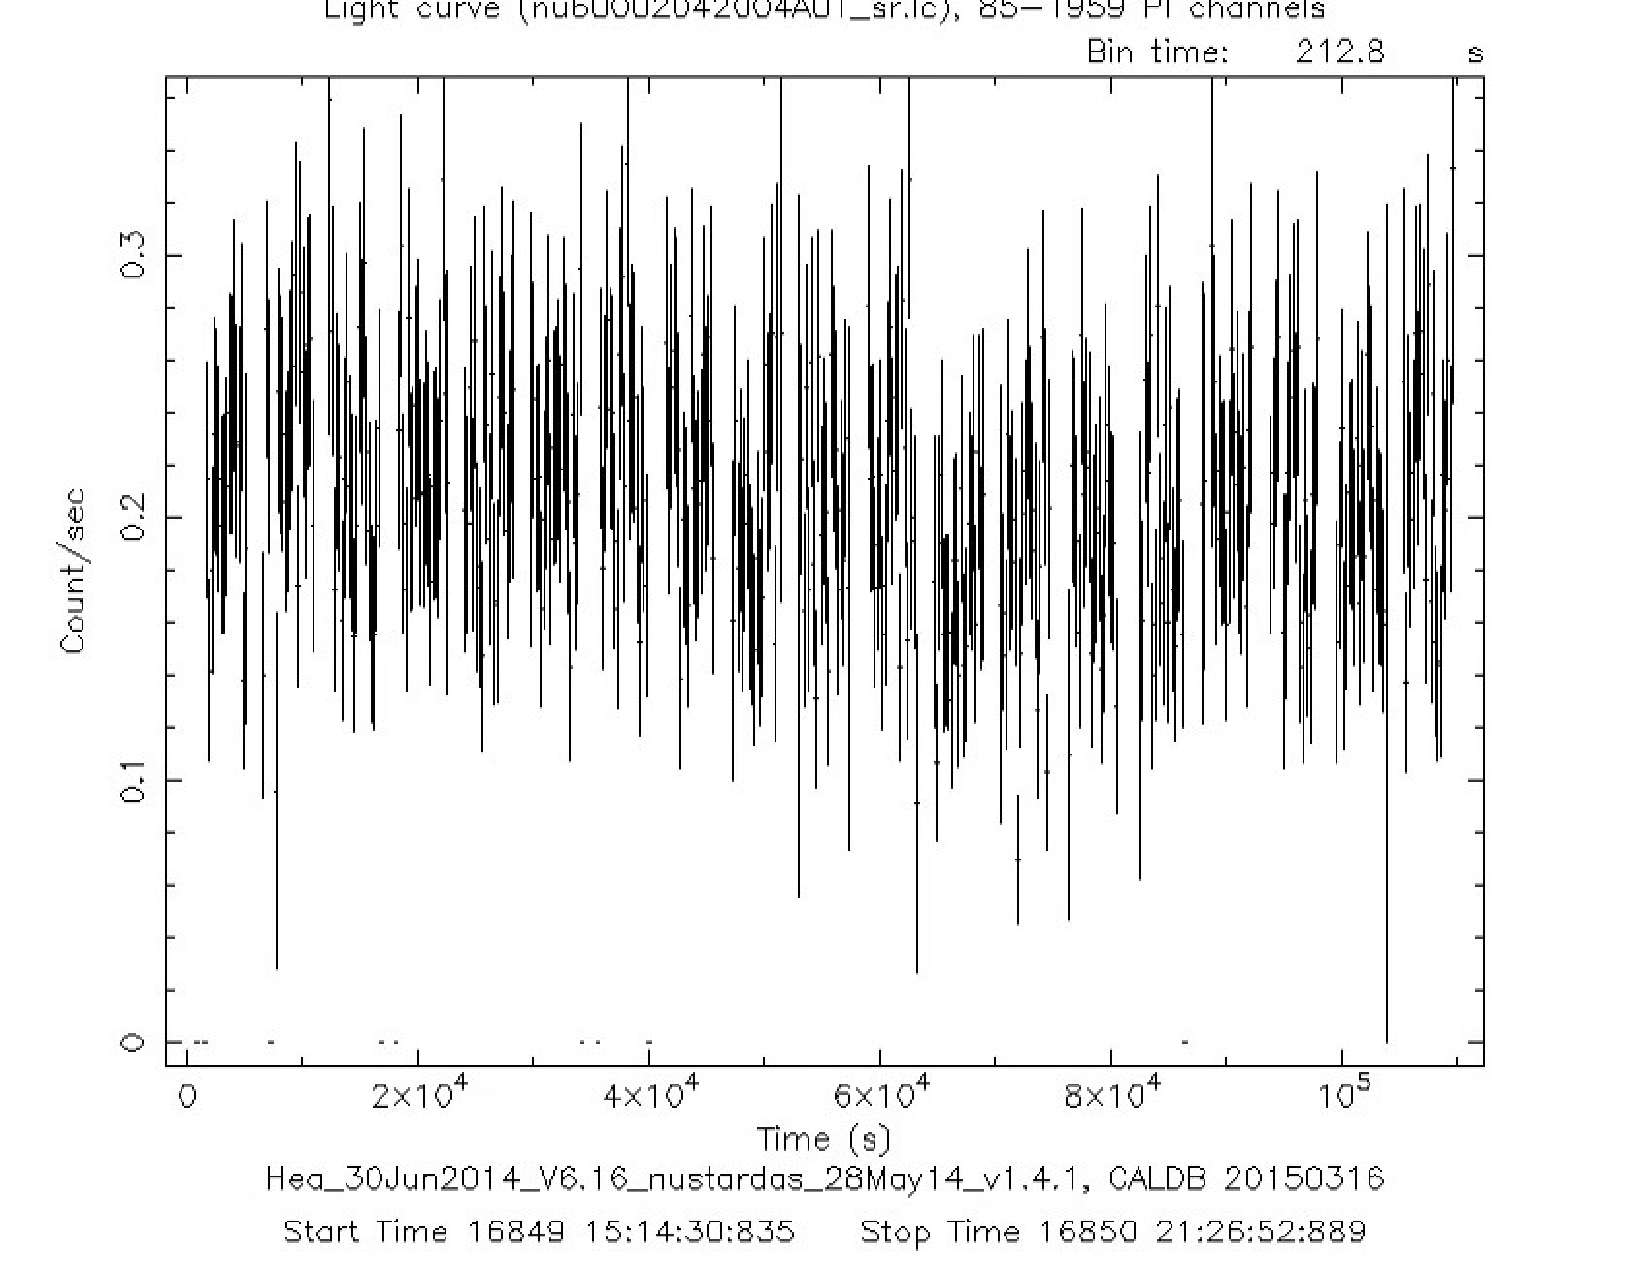
\includegraphics[width=0.7\textwidth]{Images/Light_Curve_A.pdf} 
\caption{
Energy Spectrum of NGC3516 {\it \citet{H+19}}
\label{fig:Energy_B.pdf}
}
\end{figure*}


\begin{figure*}[t]
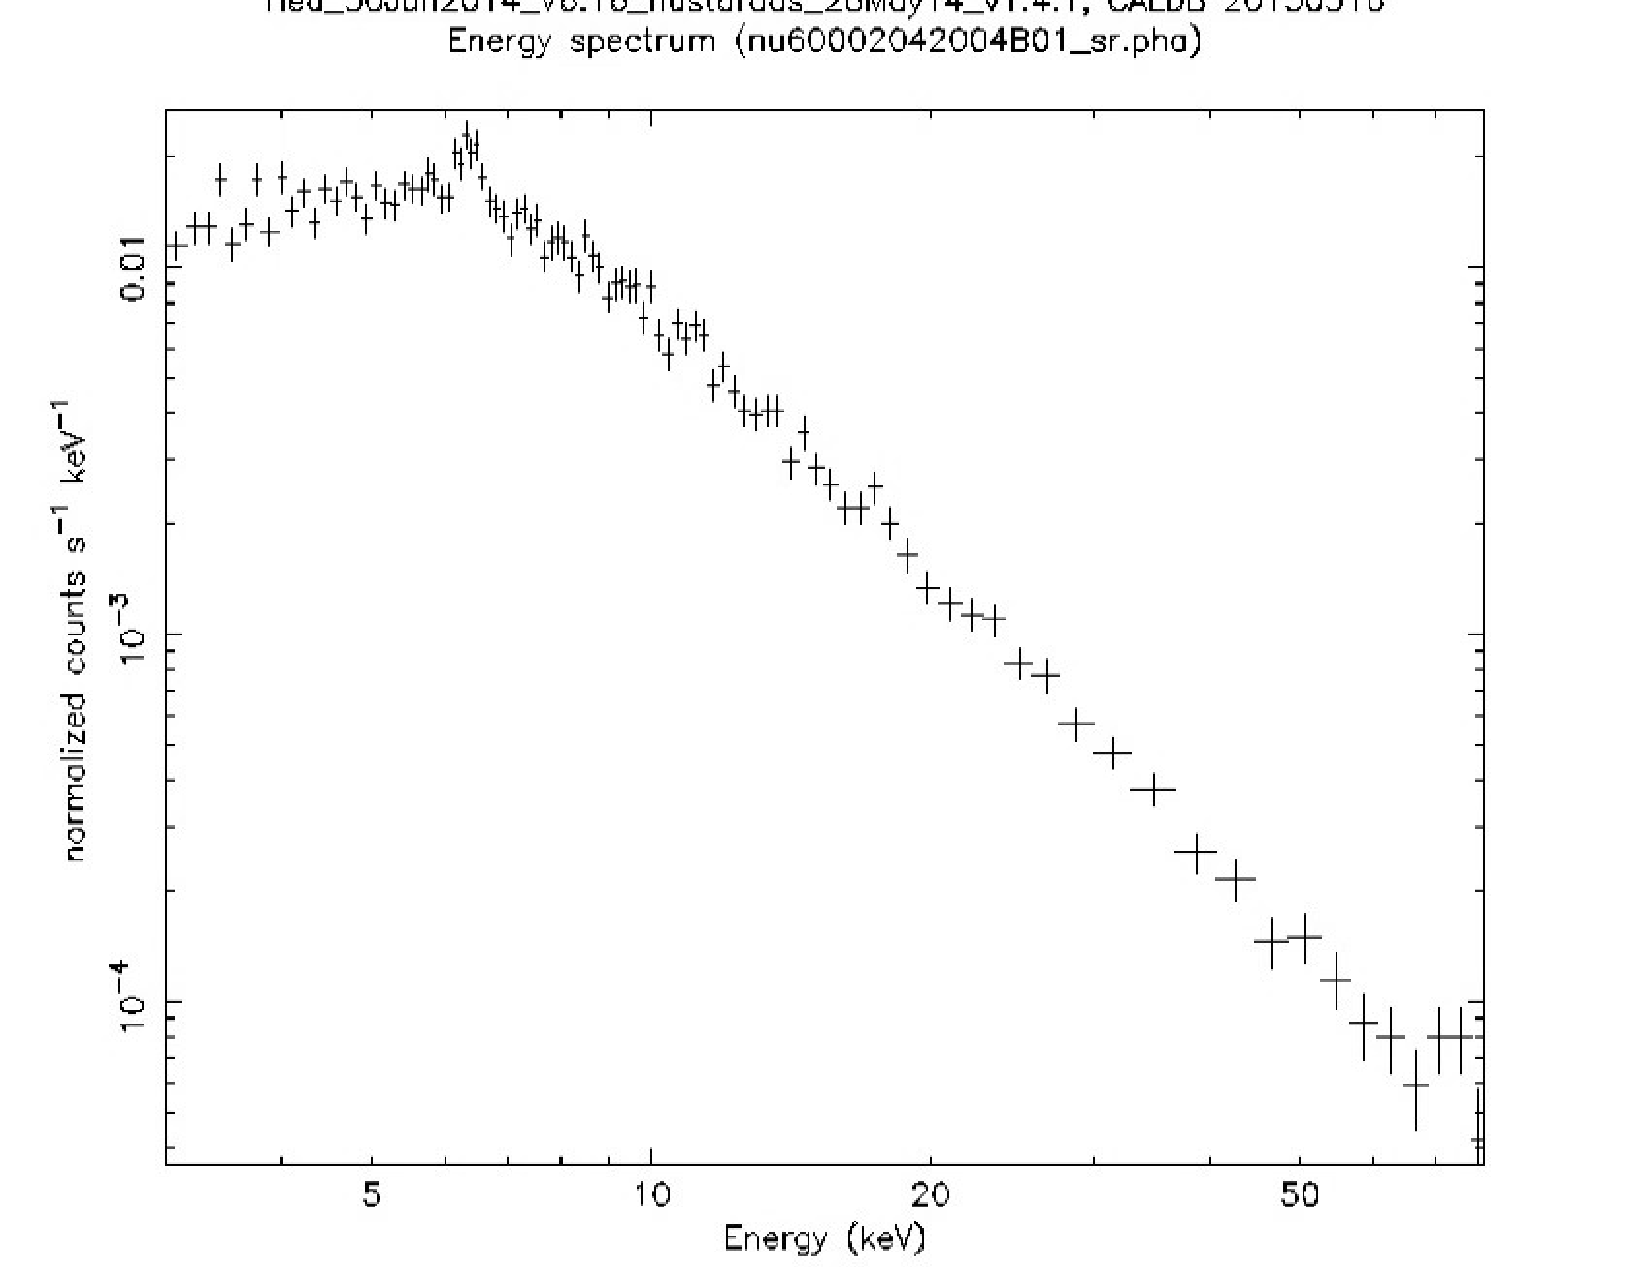
\includegraphics[width=0.7\textwidth]{Images/Light_Curve_B.pdf} 
\caption{
Light Curve of NGC3516 {\it \citet{H+19}}
\label{fig:Light_Curve_A.pdf}
}
\end{figure*}

\begin{figure*}[t]
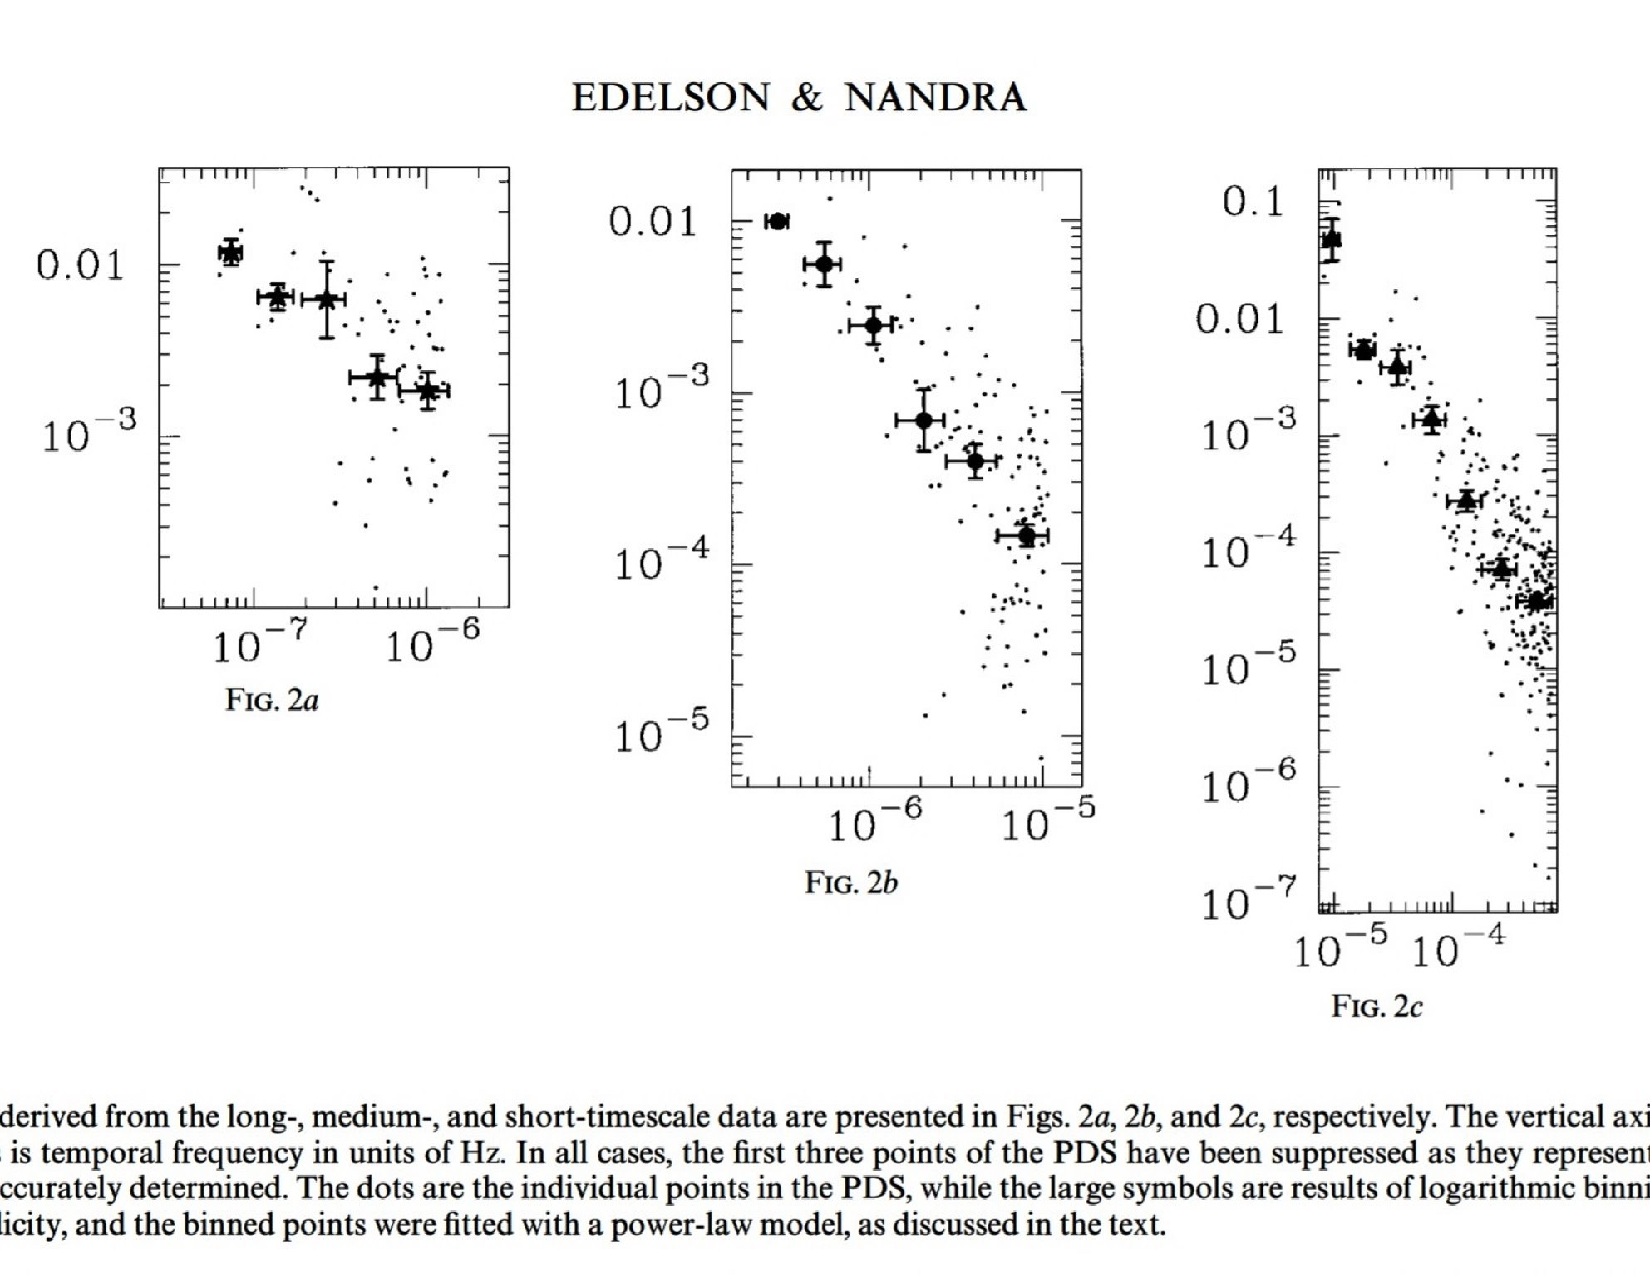
\includegraphics[width=0.8\textwidth]{Images/Elson_Image.pdf} 
\caption{
A figure taken from Edelson \& Nandra's Article showing X-Ray Variability
\label{fig:Elson_Image}
}
\end{figure*}


\subsection{Literature Review}

Active galactic nuclei are powerful concentrated regions of material surrounding black holes that are extremely luminous. While the emission spectra of these objects can be within a wide range of the electromagnetic spectrum, most AGN produce radiation peaking in the UV but with significant amounts of gamma and x-ray band emissions. They are very stable sources of luminosity and range from $10^{40}$ $ergs \times s^{-1}$ to $10^{47}$ $ergs \times s^{-1}$ {\it \citet{F+8}}.

    AGN are classified by the several types
(i) Seyfert Galaxies, which have moderate luminosities but are well understood (ii) Quasars, which are more luminous than the rest of the galaxy (iii) blazars, AGN with powerful relativistic jets of ionized material {\it \citet{F+8}} (iv) Markarian galaxies are AGN that are very luminous in the UV band (v) Radio galaxies which emit more in the optical and radio spectrums (vi) and ULIRGS which have $>10^{12} L_\odot$ in the infrared band. Interestingly enough, all of the above types can emit X-Ray radiation.

Different sub-types of AGN are usually classified by their angle of observation. For example, Seyfert I type AGN are being observed directly along the path of the central emmision. Seyfert II type AGN are those that are viewed from less direct lines of sight or from the obfuscation of the accretion disk and other material.

The effects produced by active galactic nuclei are thought to be the result of supermassive black holes accreting material from the central region of the galaxy. This typically forms an accretion disk and material will spiral inwards following a pattern determined by stellar winds and electromagnetic field. While it is not exactly known how jets are formed and material is ejected, it is generally accepted that if the stellar wind is not powerful enough to travel perpendicular to magnetic field lines, then the material will follow the magnetic field to the poles and be ejected there.

%%%%%%%%%%%%%%%%%%%%%%%%%%%%%
%%%%%%%% Methods %%%%%%%%%%%% 
%%%%%%%%%%%%%%%%%%%%%%%%%%%%%

\section{Methods/Summary}

\subsection{Data Analysis}

The data analyzed for this article was obtained through the Heasoft-6.27.2 and the NuStar datasets from the HEASARC Archive. This software was configured using packages outlined in the heasarc.gsfc.nasa.gov website documentation and the data was analyzed and processed using Heasoft FTOOLS and CALDB. The observations were made over an exposure time of 72089 s on July 11, 2014.

\subsection{Literature Review}

i. A Cutoff In The X-ray Fluctuation Power Density Spectrum Of The Seyfert 1 Galaxy NGC 3516

This paper describes the unusual X-ray fluctuations of NGC 3516 and describes them using a best fit log-log plot of fluctuation power versus frequency (Hz). It demonstrates that the fluctation strength follows a power-law distribution plus cold absorption. This article was chosen to provide more insight into the X-ray emissions of NGC 3516.

ii. Perspective: Active galactic nuclei

This source is a general and detailed overview of AGN types and characteristics. This article was chosen for the summary of AGN in the Literature Review section of this article.

iii. HEASARC Archive and NuStar data Obsid: 60002042004

Primary data source used for observations of NGC 3516 in the x-ray spectrum.

iv. The Radio Source and Bipolar Nebulosity in the Seyfert Galaxy NGC 3516

This article describes the structure of NGC 3516 in the optical and radio wave bands as well as attempting to explain some of the odd features that have formed in this galaxy.

v: Elemental Abundances in NGC 3516

An article on the material composition of NGC 3516 and the respective quantities of each element.


%%%%%%%%%%%%%%%%%%%%%%%%%%%%%
%%%%%%%% Results %%%%%%%%%%%% 
%%%%%%%%%%%%%%%%%%%%%%%%%%%%%

\section{Results/Synthesis of Work}

\subsection{Data Analysis}

The data used in this paper was collected by the Nuclear Spectroscopic Telescope Array (NuSTAR), downloaded from the NuMASTER tables on the HEASARC Archive, and was processed using Heasoft-6.27.2. The data set selected was Obsid:60002042004 and the raw data was processed using the FTOOLS nupipeline command after setting up the proper environment variables and CALDB. From there the Metrology data is processed, attitude files corrected, pixels are flagged, events are flagged, and then coordinates transformed. nupipeline is then used to screen the events and generate exposure map.

If everything has been done correctly in the previous steps, high quality data products can be extracted using the nuproducts command and by following the documentation for generating specific data sets. After corrections are applied to the products the data can be viewed in a user friendly format.

\subsection{Literature Review}

According to the observations of XMM-Newton, NGC 3516 is comprised of large amounts Nitrogen, about 2-3 times the N/H ratio of galaxies with abundant solar gases, which seems to be the case in NGC 3516. This could indicate a large stellar population of intermediate mass stars. This helps provide evidence for the X-ray model of this AGN, since the Nitrogen abundance is needed to match the spectrum observed by FUSE {\it \citet{TKM+19}}. This doesn't explain why there seem to be such strong fluctuations in the spectrum, however.

From the literature referenced in this article it is easy to see that NGC 3516 is a rather complex lenticular galaxy. The fluctuations in the x-ray spectrum seem to be extremely variable, and fluctuation power can vary by factors of about $10^3$ in the lower frequency ranges {\it \citet{EN+18}}. It is suspected that there may be active regions on certain AGN galaxies such as this one, and that as the accretion disk rotates, these active regions contribute to the variability. Other models predict that this variability is due to some process in which accretion builds up to a critical mass and then gets ejected after exceeding that limit at volatile regions that produce X-ray emissions.

From the radio source observations we know that there are some interesting features of ionization and shock wave fronts that are occurring around the outflow of the galactic nucleus {\it \citet{MWP+17}}. If these shock waves are affecting the composition of the accretion disk, then perhaps these disturbances contribute to the variability in the proposed active regions of the disk.





%%%%%%%%%%%%%%%%%%%%%%%%%%%%%
%%%%%%%% Conclusions %%%%%%%% 
%%%%%%%%%%%%%%%%%%%%%%%%%%%%%

\section{Conclusions}

NGC 3516 is a fascinatingly irregular galaxy. From its structure to the elemental composition it is highly unusual and it seems that there is a lot to be learned about x-ray fluctuations and shock wave fronts in active galaxies. 

It is possible that some of the fluctuations observed in the x-ray spectrum may be due to background sources, since this galaxy is such an extreme case it is unlikely that they affected the data much after being processed. However, since the fluctuation curve was able to mostly fit a power-law distribution, this leaves good opportunities for learning more about NGC 3516. While not all that much is known about this particular galaxy and AGNs in general, hopefully these sorts of unusual cases will teach us a lot more about how these intriguing galaxies function.



%%%%%%%%%%%%%%%%%%%%%%%%%%%%%
%%%%%%% Bibliography %%%%%%%% 
%%%%%%%%%%%%%%%%%%%%%%%%%%%%%

\pagebreak
\begin{thebibliography}{99}

\bibitem[Edelson et al.(1)]{EN+18} i. Edelson, Rick, Nandra, Kirpal, et al.\ 1999, \apj, 514: 682-690

\bibitem[Andrew C. Fabian(2)]{F+8} ii. Fabian, Andrew C.\ 1999, Proceedings of the National Academy of Sciences Vol. 96 (9) 4749-4751; DOI: 10.1073/pnas.96.9.4749

\bibitem[from NuStar, HEASARC Archive(3)]{H+19} iii. HEASARC Archive, NGC 3516 Obsid: 60002042004 NASA/Goddard Space Flight Center, Greenbelt, Maryland, 20771, USA

\bibitem[Miyaji \& Wilson et al.(4)]{MWP+17} iv. Miyaji, Takamitsu, Wilson, Andrew S., Pérez-Fournon, Ismael, et al.\ 1999, \apj, 385: 137-145

\bibitem[Turner et al.(5)]{TKM+19} v. Turner, T.J., Kraemer, S.B., 
George, I.M., Gabel, J.R., et al.\ 2003,\apj, 594: 128-135




\end{thebibliography}


%%%%%%%%%%%%%%%%%%%%%%%%%%%
%%%%% End of document %%%%%
%%%%%%%%%%%%%%%%%%%%%%%%%%%

\end{document}

